\documentclass[a4paper,12pt,twoside,openany,Seminar,chapterbib]{CMU} % HomePaper or Seminar option
\title{Online optimization for process scheduling}
\author{{JAY RASESH SHAH}}
%\rollno{12CHE1021}
%\department{Department of Chemical Engineering}
%\college{Institute of Chemical Technology}  %your college
%\address{Mumbai -- 400019}
%\degree{Bachelors of Chemical Engineering}
%\degreedate{2015 -- 2016}    %the degree date
%\guide{} %Initials of your guide

\usepackage[svgnames]{xcolor} % Required to specify font color

\usepackage{lipsum}

\usepackage{textcomp}

\usepackage{layouts}

\usepackage{epstopdf}

\usepackage[margin=1in]{geometry}

\usepackage{enumitem}

\usepackage{setspace}

\usepackage{amsmath}
\usepackage{amssymb}
%\usepackage{chemfig}
\usepackage{tikz}
\usepackage{caption}
%\usepackage{subfigure}
\usepackage{subfig}
\usepackage[pdfauthor={Jay Shah},pdftitle={Desulfurization processes and sulfur recovery},pdfkeywords={Sulfur, Desulfurization, Sulfur recovery, Claus process, MEROX, biodesulfurization, OATS process},pdfsubject={Seminar 2015-16}]{hyperref} %use [hidelinks] 

\usepackage{booktabs} %fancy tables
\usepackage{float}
\usepackage[intoc]{nomencl} %FOR NOMENCLATURE
\makenomenclature

\usepackage{pdfpages} %to insert external title page pdf

\usepackage{listings}
\usepackage{mcode}

\usepackage{rotating}
\usepackage{pdflscape}

\usepackage[version=3]{mhchem}
\usepackage{multirow}

\usepackage{tablefootnote} %allows footnotes in tables. Duh.
\usepackage{natbib}
\begin{document} 

%\pagestyle{empty} % Removes page numbers
%\renewcommand*{\thepage}{Cover}
%\includepdf{TitlePage.pdf} % includes EXTERNAL title page

\frontmatter
\tableofcontents

\listoffigures
\begingroup
\let\clearpage\relax
\vspace{3em}
\listoftables
\endgroup

\mainmatter
\chapter{Introduction}
\thispagestyle{plain}

Scheduling is a decision-making process that plays an important role in most manufacturing and service industries. %\ref{}. 
Scheduling problems arise in almost any type of industrial production facilities where given tasks need to be processes using specified resources. In a chemical process, production must be planned such that equipment, material and utilities are available at the manufacturing facility when they are needed to realize the production tasks. Production scheduling comprises the activity of planning in detail the production of a product or products in a given production facility. It boils down to the following main decisions \citep{HARJUNKOSKI2014161}:
\begin{itemize}
\item What production tasks to execute?
\item Where to process the production tasks?
\item In which sequence to produce?
\item When to execute the production tasks?
\end{itemize}

For batch processes, short-term scheduling deals with the allocation of a set of limited resources over time to manufacture one or more products following a batch recipe \citep{MENDEZ}. There has been significant development of optimization approaches to scheduling over the last two decades. The first mathematical programming approach the scheduling of multi-purpose, multi-product batch plants was proposed by \cite{KONDILI1993211}. This approach introduces the state task network (STN) representation where the process is described as a bipartite graph consisting of states and tasks.

\section{Parameter uncertainty in process scheduling}

In realistic scenarios, many of the parameters associated with scheduling are not known exactly. Parameters such as processing time, yields, prices, etc. can vary with respect to time and are subject to unexpected deviations. Robust optimization is an approach that has been suggested to mitigate these uncertainties while designing a schedule. Robust optimization seeks to generate a solution that is immune to uncertainty by ensuring that it remains feasible for all possible realizations of the uncertain parameters from within a set chosen \emph{a priori} by the modeler.

This work supports two frameworks to handle uncertainty of parameters:

\begin{itemize}
\item \textbf{Static Robust Optimization: } The first application of robust optimization in process scheduling was by \cite{LIN20041069}. This work, which utilized box uncertainty sets, was later extended by \cite{JANAK2007171} to consider uncertainty sets derived from probabilistic information. \cite{LiIerapetritou} considered box, ellipsoidal and budget uncertainty sets. All these single-stage approaches are collectively referred to as Static Robust Optimization (SRO).

\item \textbf{Adjustable Robust Optimization: } SRO approaches are generally conservative, as they assume that all of the decisions have to be made 	``here-and-now'', before the schedule begins to be implemented. In reality, many of the decisions can be ``wait-and-see'', meaning that they can be delayed until a later point when the a subset of the uncertain parameters have revealed their values. To handle such multi-stage decision making strategies, Adjustable Robust Optimization (ARO) is used, where an optimal policy is derived instead of a single, static solution. The optimal policy constitutes a family of solutions that are parameterized in the uncertain parameter realizations \citep{lappas}.

\end{itemize}•
\chapter{Problem Statement?}
\thispagestyle{plain}



\chapter{Novel desulfurization processes}
\thispagestyle{plain}

Hydrodesulfurization in combination with carbon rejection technologies, such as coking and fluid catalytic cracking (FCC) are the main technologies industrially employed for the desulfurization of crude. Although these technologies are quite capable of desulfurizing heavy oil, their carbon footprints are substantial since all of these technologies, including the production of hydrogen that is needed for HDS, involve high-temperature processing. The refining cost increases as heavier and sulfur-rich oils are being processed. Hence, alternative desulfurization pathways are of interest. In this chapter, a few non-conventional desulfurization techniques have been described.

\section{Extraction by ionic liquids}

HDS is limited due to the low conversion rates of the higher aromatics. The low sulfur limits can only be met by extreme operating conditions in terms of pressure and residence time \citep{C1GC15196G}. Hence, the process becomes uneconomic and energy inefficient. Further, in order to fulfill gasoline sulfur limits, deep desulfurization of all streams contributing to the gasoline-pool has to carried out. Although in comparison to sulfur components in diesel fuel, HDS of thiophene is reached more easily; the bottleneck of this process is the decrease in octane number due to simultaneous hydrogenation of the olefins present in the stream. In the case of diesel fuels, due to the severe HDS conditions that are necessary to produce ultra-low sulfur diesel, the cetane number is affected as well.

Liquid-liquid extraction is a technique which has been proposed for deep desulfurization because of its simplicity an and mild operating conditions. Extraction desulfurization with Ionic Liquids (ILs) as extraction solvents has the potential for alternative and future complementary technology for deep desulfurization. An ionic liquid is a non-volatile organic liquid salt, which potentially can extract sulfur and also organic nitrogen compounds in fuels by virtue of its polarity. \cite{Ito2006446} concluded that their application for desulfurization is limited due to the co-extraction of aromatic hydrocarbons. However, due to stricter environmental regulations, the aromatic hydrocarbon content (along with sulfur content) also needs to be reduced. Therefore, the co-extraction of aromatics may be an advantage since this allows for removal of both types of compounds in a single step.

\begin{figure}[t]
\centering
\fbox{\includegraphics[width=0.8\linewidth]{Images/Extractionscheme.png}}
\caption{Concept of deep desulfurization of refinery streams by extraction
with ILs \citep{B407028C}}
\label{fig:extraction}
\end{figure}

\nomenclature{IL}{Ionic Liquid}

ILs have excellent extraction properties for organic S- and N-compounds and are -- if chosen carefully -- insoluble in oils. The basic concept of such an extraction process is illustrated in Fig. \ref{fig:extraction}. \cite{C1GC15196G} have characterized the capacity and suitability of several IL solvents for thiophene and dibenzothiophene. For both sulfur aromatics, pyridinium-based ionic liquids [3-mebupy]N\ce{(CN)2} and [4-mebupy]N\ce{(CN)2}, [4-mebupy]SCN are suitable candidates since the capacity, as well as the selectivity, are higher than those of sulfolane.\footnote{Sulfolane is the commercial extraction solvent with the highest aromatic capacity, mostly used for aromatics extraction from different petroleum fractions. Hence results of ionic liquids are compared to sulfolane.} In case of the investigated imidazolium-based ionic liquids, only [BMIM]C\ce{(CN)3} fulfils the criteria and is superior to sulfolane. [BMIM]N\ce{(CN)2} only has a higher selectivity, while the selectivity of [BMIM]SCN is comparable to that of sulfolane.

Extractive desulfurization becomes increasingly difficult and unselective as the heaviness of the oil increases. Solvent loss and recovery are important detractors when desulfurizing heavy oil. The sulfur compounds are high
boiling and the heavy oil is viscous. It is unlikely that a solvent can be found that will be sulfur-selective based purely on a physical extraction. It is anticipated that any breakthrough in extractive desulfurization of heavy oil will, out of necessity, be in reactive extractive desulfurization, i.e. a solvent that chemically reacts with sulfur in sulfur-containing compounds to produce a separate phase \citep{Javadli}. Even so, this does not eliminate the problems associated with solvent recovery, which must still be addressed.

\section{Biodesulfurization}

\nomenclature{BDS}{Biodesulfurization}
\nomenclature{ODS}{Oxidative desulfurization}

Biodesulfurization is a non-invasive approach that can specifically remove sulfur from refractory hydrocarbons under mild conditions and it can be potentially used in industrial desulfurization. Intensive research has been
conducted in microbiology and molecular biology of the competent strains to increase their desulfurization activity; however, even the highest activity obtained is still insufficient to fulfill the industrial requirements. 

Sulfur forms 0.5--1\% of bacterial cell dry weight. Microorganisms require sulfur for their growth and biological activities. Sulfur generally occurs in the structure of some enzyme cofactors (such as Coenzyme A, thiamine and biotin), amino acids and proteins (cysteine, methionine, and disulfur bonds). Microorganisms, depending on their enzymes and metabolic pathways, may have the ability to provide their required sulfur from different sources. Some microorganisms can consume the sulfur in thiophenic compounds such as DBT and reduce the sulfur content in fuel. Desulfurization by microorganisms is potentially advantageous. Firstly, it is carried out in mild temperature and pressure conditions; therefore, it is considered as an energy-saving process (an advantage over HDS). Secondly, in biological activities, biocatalysts (enzymes) are involved; therefore, the desulfurization would be highly selective (an advantage over ILs).

\cite{Soleimani2007570} have described three main types of biodesulfurization:
\begin{itemize}
\item Destructive biodesulfurization
\item Anaerobic biodesulfurization
\item Specific oxidative desulfurization
\end{itemize}

Aerobic BDS was proposed as an alternative to hydrodesulfurization of crude oil. It was reported that BDS by \emph{Pantoea agglomerans} D23W3 resulted in 61\% sulfur removal from a light crude oil that originally contained 0.4\% sulfur and 63\% sulfur removal from a heavy crude oil that originally contained 1.9\% sulfur. It was found that integrated methods performed better than just BDS. By combining ODS with BDS it was possible to achieve 91\% sulfur removal from heavy oil \citep{agarwalsharma}.

The main reasons that BDS is not commercially employed for crude oil desulfurization are the low activity, the logistics of sanitary handling, shipment, storage and use of miccroorganisms within the refinery environment.

\section{Olefin alkylation of thiophenic sulfur}

The OATS process, first developed by British Petroleum, can be seen as a good alternative for the conventional desulfurization because of the comparative advantages of mild reaction conditions, no need for other reactants and minimal loss of octane number. Typically, this process consists of two steps: first, thiophene and its derivates are alkylated with the olefins in gasoline over some acidic catalysts; second, the alkylated sulfur-containing compounds are separated from gasoline by distillation. The alkylation technique is based on the concept that, when the boiling temperature of organosulfur compounds is shifted to a higher value, they can be removed from light fractions by distillation and concentrated in the heavy boiling part of the refinery streams. 

\nomenclature{OATS}{Olefin alkylation of thiophenic sulfur}

\begin{figure}[htbp]
\centering
\fbox{\includegraphics[width=\linewidth]{Images/OATS.eps}}
\caption{OATS process \citep{el2015handbook}}
\label{fig:OATS}
\end{figure}

In conventional OATS technologies, the separations and reactions are carried out with different equipment as shown in Fig. \ref{fig:OATS}. From a process intensification point of view, catalytic distillation may be more effective and economical. In the process of catalytic distillation, separation and catalytic reaction occur in the same vessel, so the conversion of the reactants can be greatly enhanced.

Using equilibrium steady state simulations, \cite{JCTB:JCTB4604} have presented a sensitivity analysis and economic evaluation of the catalytic distillation process for alkylation desulfurization of FCC gasoline.  The results indicated that the operating pressure impacts both the separation and reaction; hence increasing the operating pressure is not always beneficial to the catalytic distilation process. However, a high feed pressure is an economical option despite it having no significant effect on sulfur transfer.

A major advantage of this process is that less hydrogen is consumed since only a relatively low volume of the naphtha stream is hydrotreated. One of the disadvantages of the process is that the alkylated sulfur compounds produced require more severe hydrotreating conditions to eliminate sulfur \citep{el2015handbook}.

%\section{Oxidative desulfurization}
\chapter{GUI Design}
\thispagestyle{plain}

This chapter describes the basic structure of the instance builder web page and the various assertions and conditions required for a well defined scheduling instance.

\section{Instance structure}
To facilitate compatibility with backend C++ code, the JavaScript instance object is converted to a JSON string. JSON (JavaScript Object Notation) is a text format that is completely language independent but uses conventions that are familiar to many different programming languages, including C, C++, Java, JavaScript, Python and others. These properties make JSON an ideal data-interchange format.

JSON is built on two universal data structures:
\begin{itemize}
\item A collection of name/value pairs. In various languages, this is realized as an object, record, struct, dictionary, hash table, keyed list, or associative array.
\item An ordered list of values. In most languages, this is realized as an array, vector, list, or sequence.
\end{itemize}
Virtually all programming languages support these structures in one form or other. In JSON, they take on these forms:

An \emph{object} is an unordered set of name/value pairs. An object begins with \{ (left brace) and ends with \}  (right brace). Each name is followed by \lstinline{:} (colon) and the name/value pairs are separated by \lstinline{,} (comma).
\section{Instance object}
\label{instanceCompletion}
\begin{figure}[htbp]
\begin{center}
\begin{lstlisting}[xleftmargin=.2\textwidth, xrightmargin=.2\textwidth]
{
	"Name": "Scheduling_Instance",
	"Horizon": 8,
	"Units": [],
	"States": [],
	"Orders": [],
	"Utilities": [],
	"Tasks": [],
	"isCompleteInstance": false
}
\end{lstlisting}\end{center}•
\caption{Instance JSON}
\label{code:Instance}
\end{figure}•
The structure of the Instance JSON object is as shown in Figure \ref{code:Instance}. The empty arrays \lstinline{[]} for \lstinline{"Units"}, \lstinline{"States"}, \lstinline{"Tasks"}, \lstinline{"Utilities"} and \lstinline{"Orders"} in the structure contain the JSON objects as specific to the instance. \lstinline{"Name"} is a string denoting the given name for the instance. \lstinline{"Horizon"} is an integer or float. \lstinline{"isCompleteInstance"} is a boolean \lstinline{true} or \lstinline{false} value denoting if an instance is completely specified.

Figures \ref{fig:unitJSON} - \ref{fig:taskJSON} show the structures of the unit, state, utility, order and task JSON objects respectively.
\begin{figure}[!tbp]
  \centering
  \begin{minipage}[b]{0.4\textwidth}
    \begin{lstlisting}
{
	"Name": "Unit1",
	"MaximumCapacity": 100
}
\end{lstlisting}
    \caption{Unit JSON object}
\label{fig:unitJSON}
  \end{minipage}
  \hfill
  \begin{minipage}[b]{0.4\textwidth}
    \begin{lstlisting}
{
	"StateName": "State1",
	"StateInitialLevel": 100,
	"StateMaxLevel": 100,
	"IsZeroWait": true,
	"IsUIS": false,
	"Price": 10
}
\end{lstlisting}
    \caption{State JSON object}
  \end{minipage}
\end{figure}

\begin{figure}[!tbp]
  \centering
  \begin{minipage}[b]{0.4\textwidth}
\begin{lstlisting}
{
	"Name": "Utility1",
	"MaximumAvailability": 250
}
\end{lstlisting}
    \caption{Utility JSON object}
\label{fig:utilityJSON}
  \end{minipage}
  \hfill
  \begin{minipage}[b]{0.4\textwidth}
\begin{lstlisting}
{
	"StateName": "Product1",
	"Amount": 100
}
\end{lstlisting}
    \caption{Order (demand) JSON object}
  \end{minipage}
\end{figure}

An instance is deemed `complete' if:
\begin{enumerate}
\item At least one valid unit
\begin{itemize}
\item Positive maximum capacity
\end{itemize}
\item At least two states
\begin{itemize}
\item Non-negative maximum capacity
\item Initial level is less than or equal to maximum capacity
\item At least one state with positive initial level
\end{itemize}
\item At least one valid task
\begin{itemize}
\item At least one compatible unit with non-zero processing time (at least one of $\alpha$ or $\beta$ is non-zero)
\item At least one consumed state
\item At least one produced state
\end{itemize}
\item Positive horizon and at least one state to be sold with positive price OR At least one state in demand with positive demand amount
\end{enumerate}



%\subsection{Tasks}
\begin{figure}[htbp]

\begin{lstlisting}[xleftmargin=.2\textwidth, xrightmargin=.2\textwidth]
{
	"TaskName": "Task1",
	"CompatibleUnits": [
		{
		"UnitName": "Unit1",
		"alpha": 5,
		"beta": 1
		}
	],
	"ConsumedStates": [
		{
		"ConStateName": "State1",
		"consRatio": 1
		}
	],
	"ProducedStates": [
		{
		"ProdStateName": "State2",
		"prodRatio": 1
		}
	],
	"ConsumedUtilities": [
		{
		"ConsUtilName": "Utility1",
		"CompUnit": "Unit1",
		"gamma": 2,
		"delta": 0.2
		}
	]
}
\end{lstlisting}
\caption{Task JSON object}
\label{fig:taskJSON}
\end{figure}•


\section{Overall scheduling process flow}
\begin{figure}[htbp]
\centering
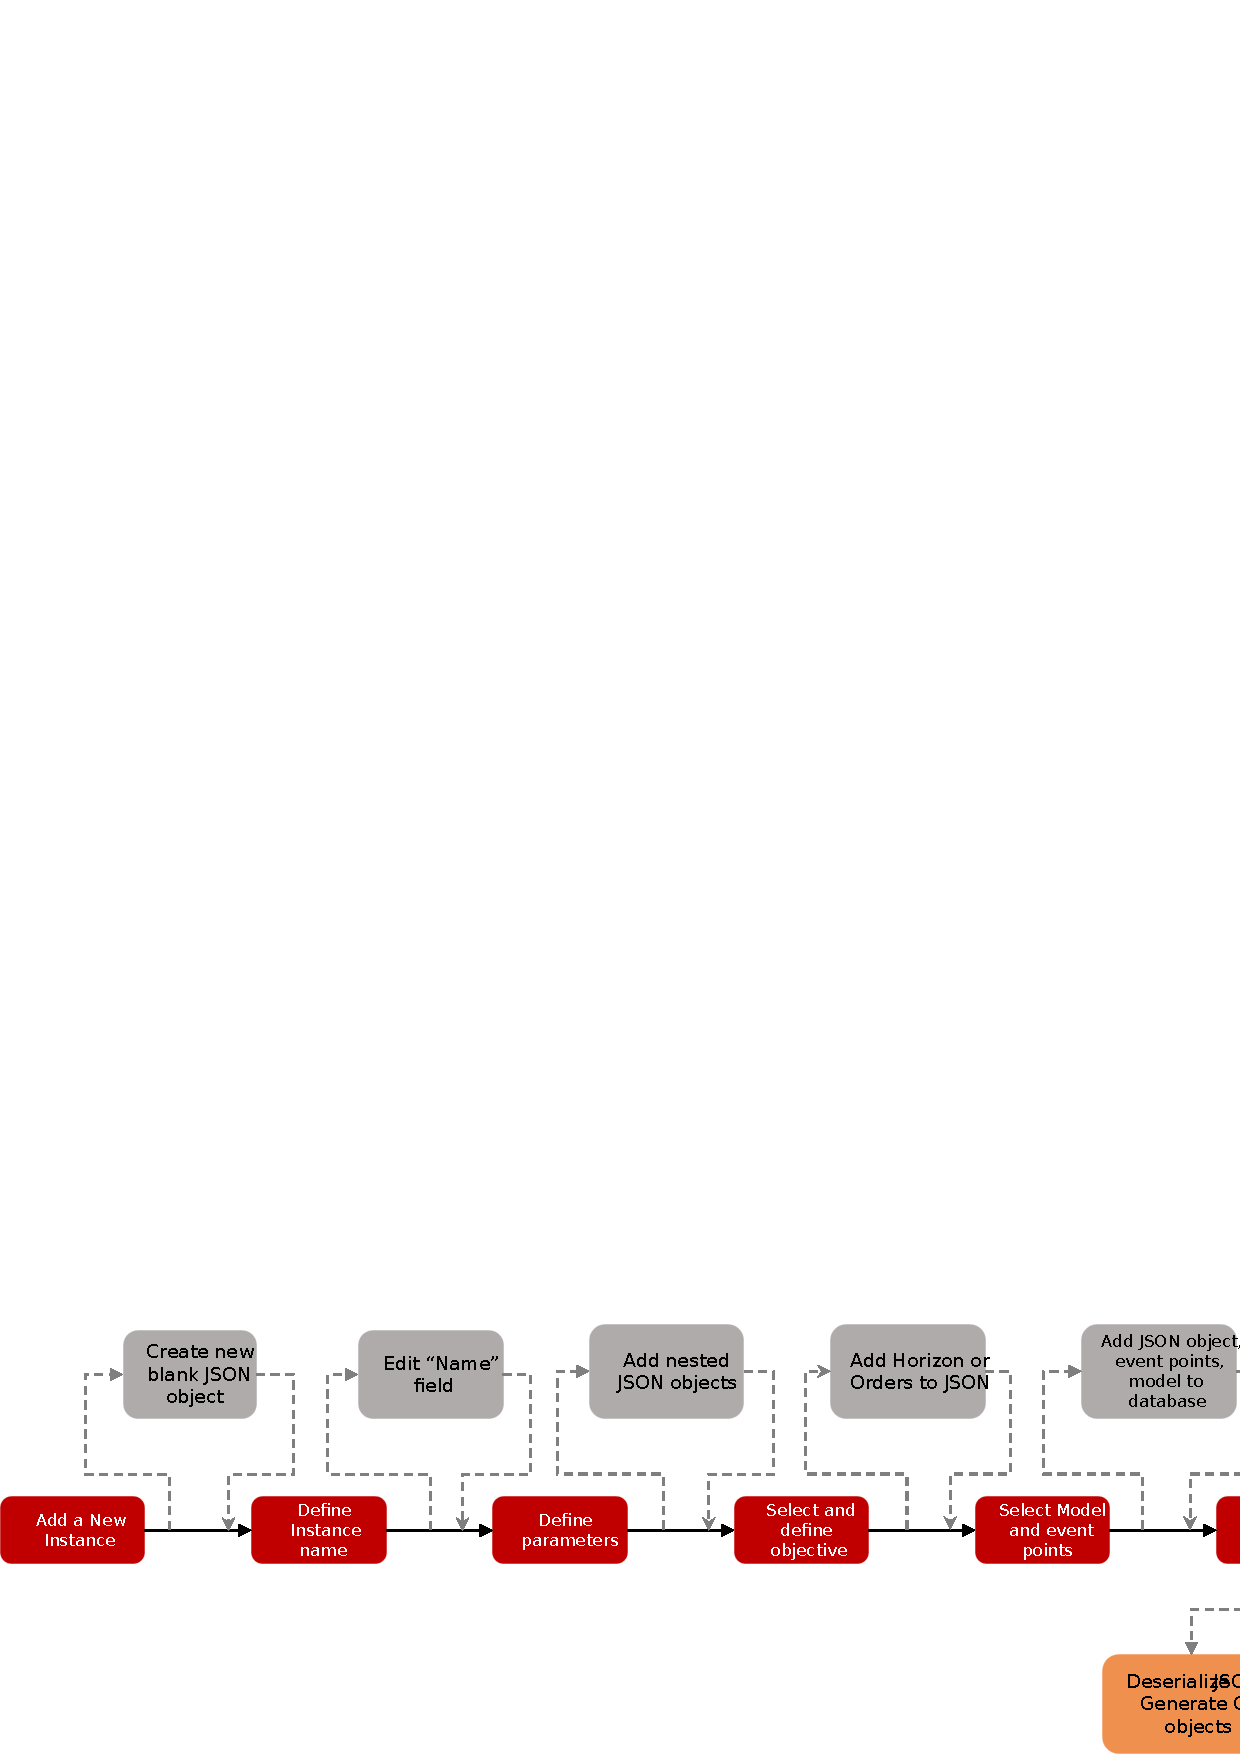
\includegraphics[width=\linewidth]{Images/Communication.png}
\caption{Overall process flow}
\label{fig:Communication}
\end{figure}

Figure \ref{fig:Communication} shows the underlying process behind creating and submitting a scheduling instance. At each stage of the instance building process, the JSON object is converted to a string by means of the \texttt{JSON.stringify()} method in JavaScript and saved in a backend mySQL database. A more detailed process flow for parameter and objective input is shown in Fig. \ref{fig:paraminput}. Once the the instance is complete and amenable to optimization, in the deterministic version, the user has the option of selecting the number of event points and scheduling model to be used. In the uncertain version, the user has additional choices to select uncertain parameters and adjustable variables.

\begin{figure}[htbp]
\centering
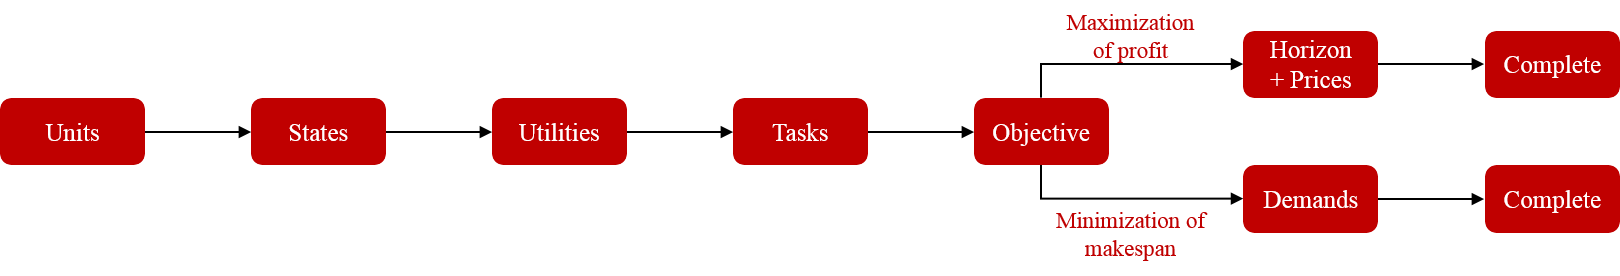
\includegraphics[width=\linewidth]{Images/ParameterObjectiveInput.png}
\caption{Parameter and objective input}
\label{fig:paraminput}
\end{figure}

On submitting, a C++ JSON deserializer converts the JSON string to C++ objects. These are then used to build a mixed-integer model in CPLEX according to the model specified by the user.

On successful completion, the following statistics are displayed on the results page:
\begin{itemize}
\item Run time
\item Forumlation
\item Number of event points
\item Objective type
\item Solver status
\item Objective value
\item Number of constraints
\item Number of binary variables
\item Number of continuous variables
\item Number of continuous variables
\item Nodes
\item Root node relaxation
\item Relative gap (\%)
\end{itemize}

If the user has elected to incorporate uncertainty into the instance, the following additional information is displayed:
\begin{itemize}
\item Uncertain Parameter(s)
\item Level of uncertainty
\item Adjustable Variable(s)
\end{itemize}

Additionally, a Gantt chart for the optimal schedule and material inventory charts are displayed. If utilities are specified by the user, then a utility consumption plot is also displayed.

\section{Instance builder}

\begin{figure}[htbp]
\centering
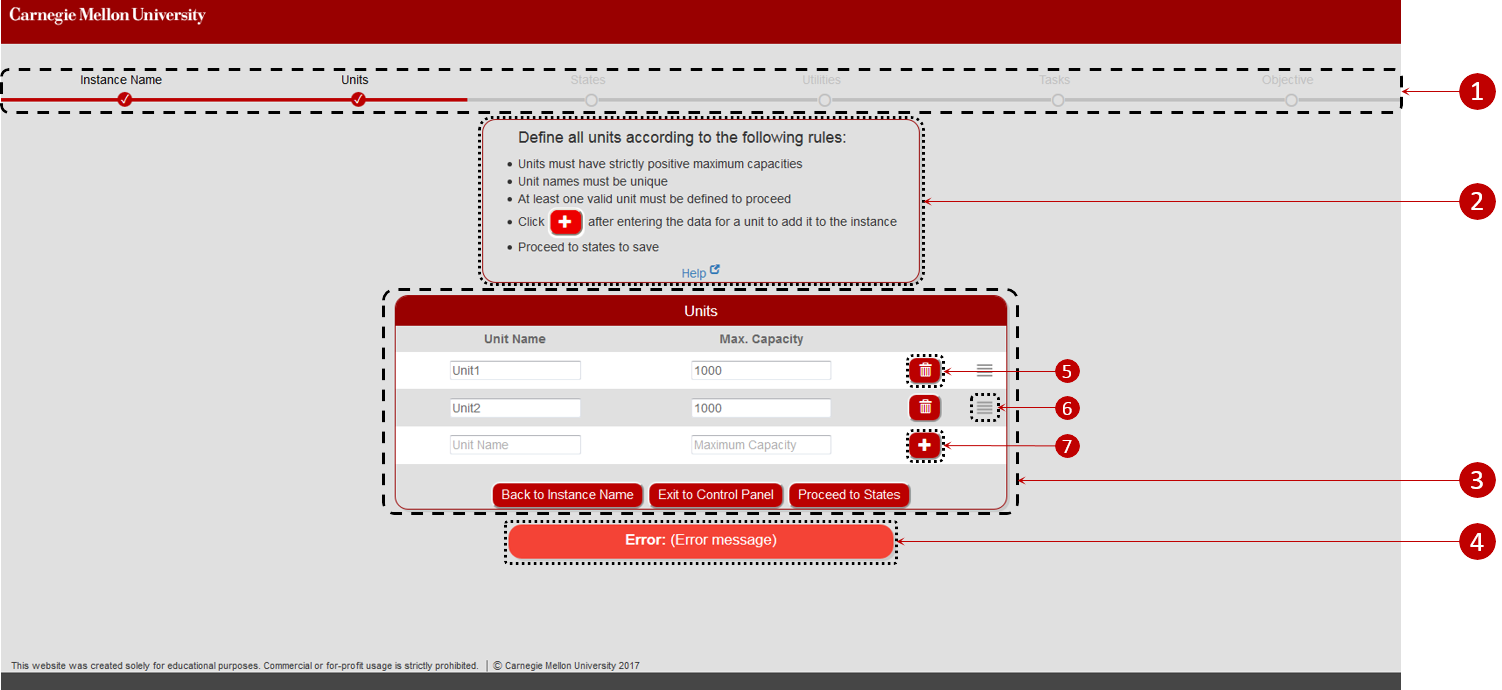
\includegraphics[width=\linewidth]{Images/GUIDesign.png}
\caption[Instance builder elements]{Instance builder elements:
1. Progress bar
2. Instructions
3. Input table
4. Error message(s)
5. Delete item 
6. Drag and drop to rearrange
7. Add new item}
\label{fig:IBGUI}
\end{figure}

Figure \ref{fig:IBGUI} shows the elements in the instance builder GUI. The screenshot in the figure shows the elements in the Units input table. The structure of the States, Utility and Tasks input table follows the same structure. A progress tracker is provided to track the status of the instance being edited. 

Error messages are displayed to ensure that the user input is valid and the instance completion criteria listed in section \ref{instanceCompletion} are satisfied.
 Once a particular set of inputs is completed, clicking on the proceed button will display the next input table.






\section{Submission page}

\begin{figure}[htb]
\centering
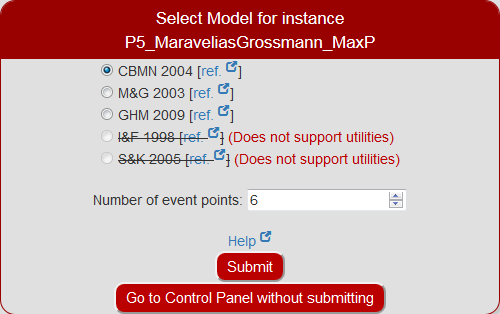
\includegraphics[width=0.8\linewidth]{Images/SelectModelUtilities.png}
\caption{Model selection table for an instance involving utilities}
\label{fig:selectModel}
\end{figure}

On successful completion, an instance becomes available for submission. A screenshot of the model selection table is shown in Fig. \ref{fig:selectModel}. The CBMN 2004 model is selected by default for both the deterministic and uncertain versions. The I\&F 1998 and S\&K 2005 models do not support instances with utilities involved.

\subsection{Uncertainty frameworks}

If the user elects to incorporate uncertainty in the instance, four types of uncertain variables are available:
\begin{enumerate}
\item Fixed processing time ($\alpha$)
\item Fixed and variable processing time ($\alpha + \beta$)
\item Task yield ($\rho_p$)
\item Fixed processing time and task yield ($\alpha + \rho_p$)
\end{enumerate}

The availability of SRO and ARO frameworks for each of the sets of uncertain variables is shown in Table \ref{tab:adjvars}. If ARO is selected, the uncertain parameters selected dictate the availability of adjustable variables.

\begin{table}[htb]
\centering
\caption{Uncertainty frameworks and  adjustable variables}
\label{tab:adjvars}
\begin{tabular}{@{}cccccc@{}}
\toprule
                  & \multicolumn{2}{c}{Frameworks} & \multicolumn{3}{c}{Adjustable variables} \\ \cmidrule(l){2-6} 
Uncertain parameters   & SRO        & ARO        & \phantom{S } T \phantom{ S}            & \phantom{S } S \phantom{ S}           & B + S       \\ \midrule
$\alpha$          & \checkmark & \checkmark & \checkmark   & \xmark      & \checkmark  \\
$\alpha + \beta$  & \checkmark & \checkmark & \checkmark   & \xmark      & \xmark      \\
$\rho_p$          & \xmark     & \checkmark & \xmark       & \checkmark  & \xmark      \\
$\alpha + \rho_p$ & \xmark     & \checkmark & \checkmark   & \checkmark  & \xmark      \\ \bottomrule
\end{tabular}
\end{table}
\chapter{Case Study}
\thispagestyle{plain}

\section{Instance description}
In this chapter, we present a case study of a well known scheduling instance from \cite{KONDILI1993211}, optimized for the deterministic case using the described online tool. The production of two products 1 and 2 from three feed stocks A, B and C takes place according to the STN representation given in Fig. \ref{fig:STN}. This instance has four intermediate states and five tasks.

\begin{figure}[htbp]
\centering
\fbox{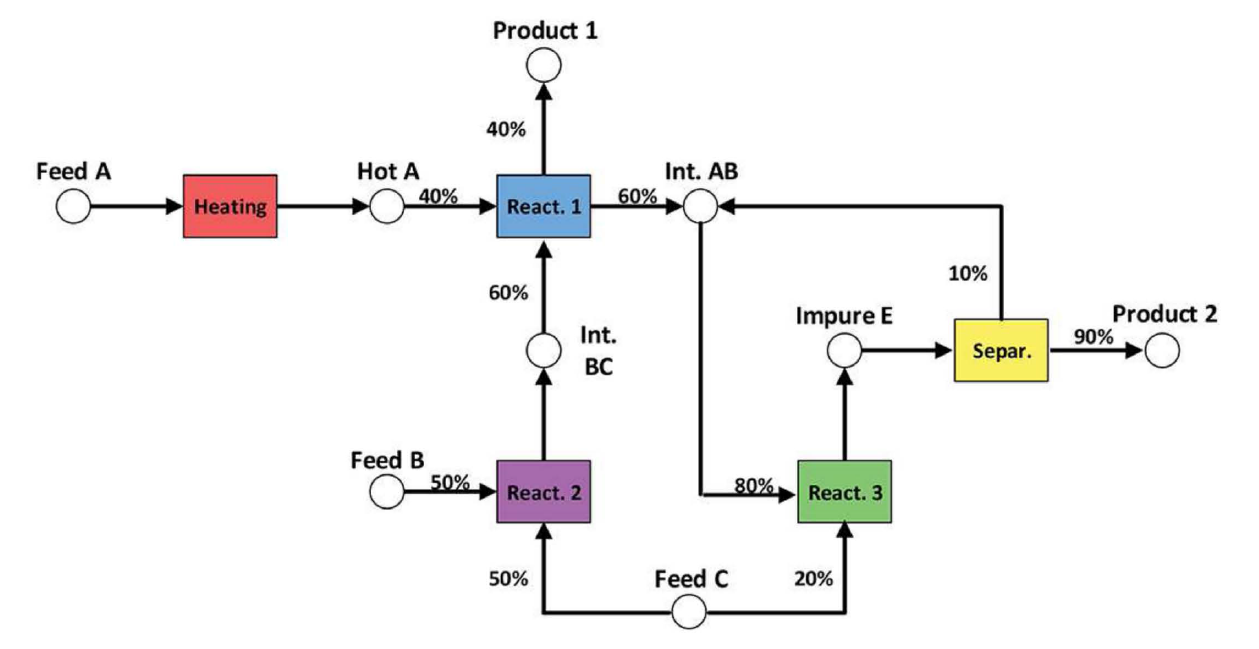
\includegraphics[width=\linewidth]{Images/STN.png}}
\caption{State task network for the example instance}
\label{fig:STN}
\end{figure}

Table \ref{tab:statelevels} shows the state maximum capacity and initial load data for the problem. The available unit, task compatibility and processing time data is given in Table \ref{tab:tasks}.

\begin{table}[htb]
\centering
\caption{Problem data (states)}
\label{tab:statelevels}
\begin{tabular}{@{}cccc@{}}
\toprule
\textbf{State} & \textbf{Capacity} & \textbf{Initial load} & \textbf{Price (per unit)} \\ \midrule
Feed A         & 1000              & 1000                  & -                         \\
Feed B         & 1000              & 1000                  & -                         \\
Feed C         & 1000              & 1000                  & -                         \\
Hot A          & 100               & -                     & -                         \\
Int. BC        & 200               & -                     & -                         \\
Int. AB        & 150               & -                     & -                         \\
Impure E       & 200               & -                     & -                         \\
Product 1      & 1000              & -                     & 10                        \\
Product 2      & 1000              & -                     & 10                        \\ \bottomrule
\end{tabular}
\end{table}

\begin{table}[htb]
\centering
\caption{Problem data (units \& tasks)}
\label{tab:tasks}
\begin{tabular}{@{}ccccccccc@{}}
\toprule
Unit         & \multicolumn{2}{c}{Heater} & \multicolumn{2}{c}{Reactor 1} & \multicolumn{2}{c}{Reactor 2} & \multicolumn{2}{c}{Separator} \\ \cmidrule(l){2-9} 
Maximum Load & \multicolumn{2}{c}{100}    & \multicolumn{2}{c}{50}        & \multicolumn{2}{c}{80}        & \multicolumn{2}{c}{200}       \\ \midrule
Tasks        & $\alpha$       & $\beta$       & $\alpha$         & $\beta$        & $\alpha$         & $\beta$        & $\alpha$         & $\beta$        \\ \cmidrule(l){2-9} 
Heating      & 0.667        & 0.007       &                &              &                &              &                &              \\
Reaction 1   &              &             & 1.334          & 0.027        & 1.334          & 0.017        &                &              \\
Reaction 2   &              &             & 1.334          & 0.027        & 1.334          & 0.017        &                &              \\
Reaction 3   &              &             & 0.667          & 0.013        & 0.667          & 0.008        &                &              \\
Separation   &              &             &                &              &                &              & 1.334          & 0.007        \\ \bottomrule
\end{tabular}
\end{table}

\section{Defining instance parameters}
\subsection{Defining units}
\begin{figure}[htb]
\centering
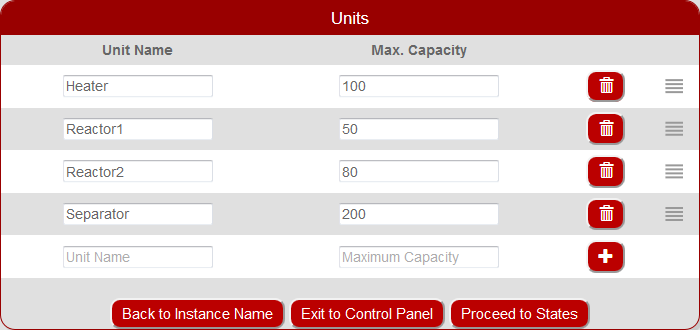
\includegraphics[width=\linewidth]{Images/DefineUnits.png}
\caption{Units input into webtool}
\label{fig:defUnits}
\end{figure}
Unit names and maximum capacities from Table \ref{tab:tasks} are input into the units table of the web tool as shown in Fig. \ref{fig:defUnits}.



\subsection{Defining states}
\begin{figure}[htbp]
\centering
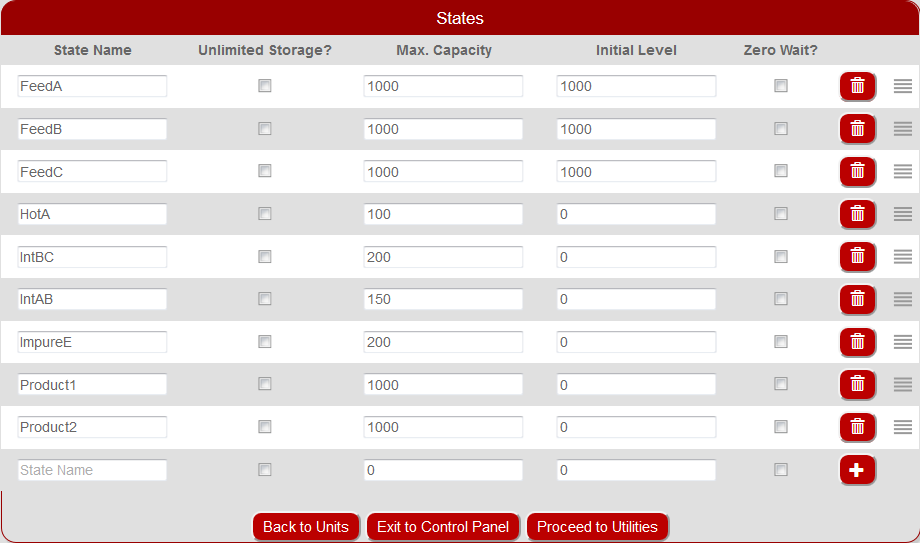
\includegraphics[width=\linewidth]{Images/DefineStates.png}
\caption{States input into webtool}
\label{fig:defStates}
\end{figure}
State names, maximum storage capacities and initial levels from Table \ref{tab:statelevels} are input into the units table of the web tool as shown in Fig. \ref{fig:defStates}.


\subsection{Defining tasks}
\begin{figure}[htb]
\centering
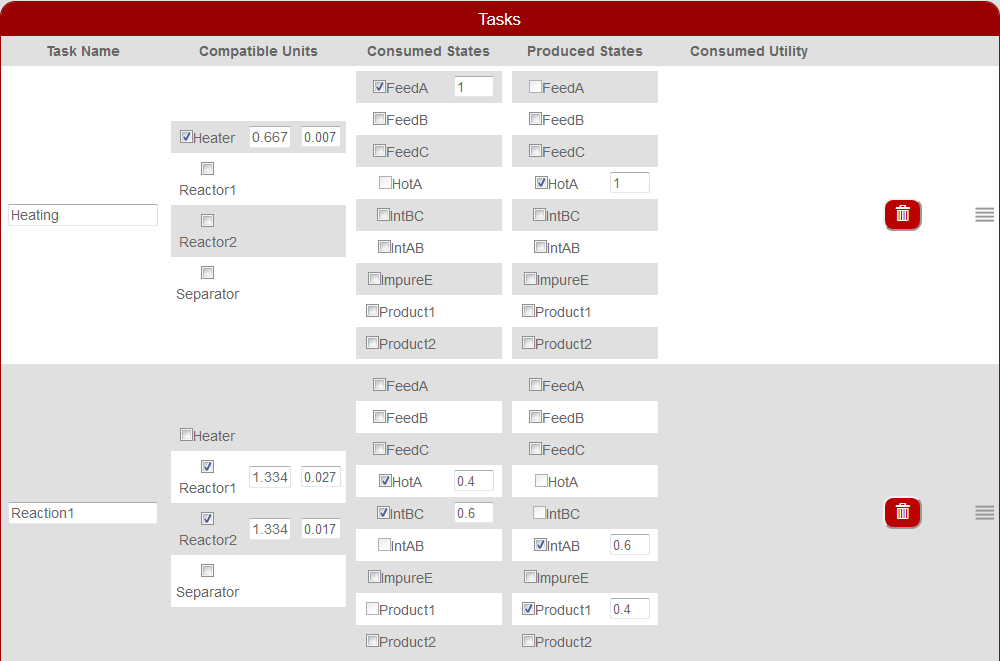
\includegraphics[width=\linewidth]{Images/DefineTasks.png}
\caption{Tasks input into webtool}
\label{fig:defTasks}
\end{figure}

This instance does not involve utilities. Hence we can skip utilities input. For each task in Table \ref{tab:tasks}, the values of $\alpha$ and $\beta$ are input after selecting the appropriate compatible unit(s). Fig. \ref{fig:defTasks} shows the tasks table after successful input of tasks Heating and Reaction 1.


\subsection{Objective}

\begin{figure}[htb]
\centering
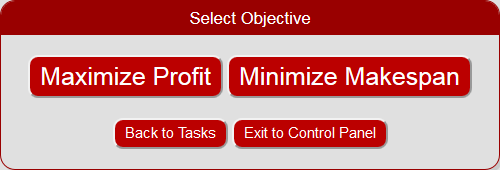
\includegraphics[width=0.8\linewidth]{Images/DefineObjective.png}
\caption{Objective selection}
\label{fig:selectObjective}
\end{figure}

For this case, we will consider the case of maximization of profit. After successful completion of the tasks input, the objective selection options are available as shown in Fig. \ref{fig:selectObjective}. After clicking on ``Maximize profit'', the horizon and price input screen appears as shown in Fig. \ref{fig:prices}. The instance definition is complete after input of horizon and price data for Product 1 and Product 2 from Table \ref{tab:statelevels}. We will consider an 8 hour horizon for this case study.

\begin{figure}[htb]
\centering
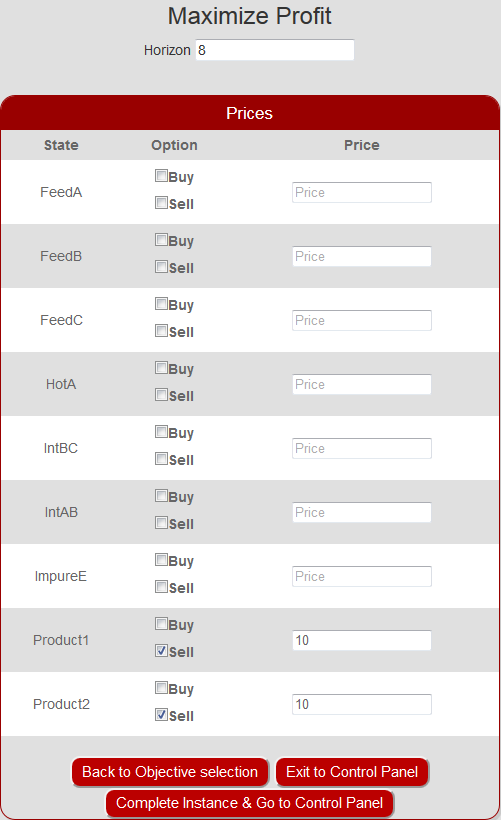
\includegraphics[width=0.8\linewidth]{Images/Prices.png}
\caption{Horizon and price input}
\label{fig:prices}
\end{figure}

\subsection{Model and event points}







%------------------------------------------------------------------------------------------------
% FOR NOMENCLATURE
%------------------------------------------------------------------------------------------------
%1. COMPILE NORMALLY
%2. GO TO CMD PROMPT, CHANGE DIRECTORY TO FOLDER
%3. TYPE makeindex Seminar.nlo -s nomencl.ist -o Seminar.nls
%4. COMPILE AGAIN
%------------------------------------------------------------------------------------------------

%\appendix

%\chapter{Temperature-Enthalpy plot} % Main appendix title

\label{AppendixA} % For referencing this appendix elsewhere, use \ref{AppendixA}

The following program was used to plot the emperature-enthalpy graph in section \ref{sec:tempenthalpy} (Fig. \ref{pinch}):
\lstinputlisting[language=Python]{Appendices/Pinch_v2.py}
%\chapter{Absorption section process flow diagram} % Main appendix title
\begin{figure}[t]
\centering
\fbox{\includegraphics[width=\linewidth]{Images/Absorption.eps}}
\caption{Absorption section}
\label{absorption}
\end{figure}
\label{AppendixB} % For referencing this appendix elsewhere, use \ref{AppendixB}





\backmatter
\def\nomname{Abbreviations}
\printnomenclature[3cm]
%\addcontentsline{toc}{chapter}{Nomenclature}
\newpage

%\singlespacing
\setlength{\bibhang}{7mm}
\bibliographystyle{ICTv2}
\bibliography{Bibliography/bibtexdb}
%\nocite{*}

\end{document}